\documentclass[final]{beamer}

% ====================
% Packages
% ====================

\usepackage[T1]{fontenc}
\usepackage{lmodern}
\usepackage[french=quotes]{csquotes} \MakeOuterQuote{"}
\usepackage[orientation=portrait,size=a0,scale=1.0]{beamerposter}
\usetheme{gemini}
\usecolortheme{nott}
\usepackage{graphicx}
\usepackage{booktabs}
\usepackage{tikz}
\usepackage{multicol}
\usepackage{pgfplots}
\usepackage[inkscapeformat=png]{svg}
\pgfplotsset{compat=1.14}
\usepackage{anyfontsize}
\usepackage{xcolor}
\usepackage[skip=2pt,font=normalsize]{subcaption}
\usepackage{adjustbox}
\usepackage{tabularx}
\usepackage{caption}
\usepackage{changepage}
\usepackage[english]{babel}
\captionsetup{font=it}

% \setbeamersize{text margin left=30mm,text margin right=30mm} 

% \addtobeamertemplate{block begin}{%
%   \setlength{\textwidth}{1.2\textwidth}%
%   \leftskip=10pt\rightskip=10pt\vspace{10pt}
%   \par\vspace{10pt}
% }{}


% \setbeamertemplate{itemize/enumerate body begin}{\normalsize}
% \setbeamertemplate{itemize/enumerate subbody begin}{\normalsize}
% \setbeamertemplate{itemize/enumerate subsubbody begin}{\normalsize}

\usepackage{tikz}
\usetikzlibrary{shapes.geometric, arrows}

% Defining Tickz Style
\tikzstyle{startstop} = [rectangle, rounded corners, minimum width=3cm, minimum height=1cm, text centered, text width=10cm, draw=white, fill=white]

% \tikzstyle{io} = [trapezium, trapezium left angle=70, trapezium right angle=110, minimum width=3cm, minimum height=1cm, text centered, text width=4.5cm, draw=black, fill=blue!30 ]

\tikzstyle{process} = [rectangle, minimum width=3cm, minimum height=1cm, text centered, text width=6cm, draw=black, fill=white, text width=10cm]

% \tikzstyle{decision} = [diamond, minimum width=3cm, minimum height=1cm, text centered, draw=black, fill=green!30]

\tikzstyle{arrow} = [ultra thick,->,>=stealth]


% ====================
% Lengths
% ====================

% If you have N columns, choose \sepwidth and \colwidth such that
% (N+1)*\sepwidth + N*\colwidth = \paperwidth
\newlength{\sepwidth}
\newlength{\colwidth}
\setlength{\sepwidth}{-2ex}
\setlength{\colwidth}{0.45\paperwidth}

\newcommand{\separatorcolumn}{\begin{column}{\sepwidth}\end{column}}


\newenvironment{variableblock}[3]{%
  \setbeamercolor{block body}{#2}
  \setbeamercolor{block title}{#3}
  \begin{block}{#1}}{\end{block}}

\addtobeamertemplate{block begin}
  {
  \setlength{\textwidth}{1.07\textwidth}%
  }
  {%\vspace{1ex plus 0.5ex minus 0.5ex} % Pads top of block
     % separates paragraphs in a block
   %\setlength{\parskip}{24pt plus 1pt minus 1pt}%
   \begin{adjustwidth}{0.5cm}{0.5cm}
}
\addtobeamertemplate{block end}
  {\end{adjustwidth}%
   \vspace{1ex plus 0.5ex minus 0.5ex}
   }% Pads bottom of block
  {}
  %{\vspace{10ex plus 1ex minus 1ex}} % Seperates blocks from each other

% ====================
%Title
% ====================

\title{On the Organization of a Multi-Agent System for Cyber-defense}

\author{\textbf{Julien Soulé} \inst{1,2} \and Jean-Paul Jamont \inst{1} \and Michel Occello \inst{1} Paul Théron \inst{3} Louis-Marie Traonouez \inst{2}}

\institute[shortinst]{\inst{1} Univ. Grenoble Alpe, Grenoble INP, LCIS, Valence, France \samelineand \inst{2} Thales Land and Air Systems, BL IAS, Rennes, France \samelineand \inst{3} AICA IWG, La Guillermie, France}


% ====================
% Footer (optional)
% ====================

\footercontent{
% \href{https://www.lipsum.com}{\textbf{https://www.lipsum.com}} \hfill

% \raggedleft

% \textbf{Ph.D. Connect Conclave 2023} \hfill

\textbf{\underline{Contact:}} \ \href{mailto:julien.soule@lcis.grenoble-inp.fr}{\textit{julien.soule@lcis.grenoble-inp.fr}}}
% (can be left out to remove footer)


\logoright{
\includegraphics[height=3cm]{logos/grenoble-inp_logo.png}}
{
\includegraphics[height=2cm]{logos/lcis_logo.png}}
{
\includegraphics[height=3.5cm]{logos/uga_logo.jpg}}
{
\includegraphics[height=3.5cm]{logos/la-ruche_logo.png}}


\begin{document}

\begin{frame}[t]

\vspace{-2ex}


\begin{columns}[t]
\separatorcolumn

\hspace{-1ex}

\begin{column}{\colwidth}

\begin{variableblock}{Context}{bg=lightgray,fg=black}{bg=lightgray,fg=black}

\begin{itemize}

    \item \headingNoLine{Systems with important attack surface}
    \begin{itemize}
        \item Connected objects (IoT/IoBT), drones, home automation, all-terrain vehicles, etc.
        \item Cyber, heterogeneous and distributed infrastructures
    \end{itemize}

    \item \headingNoLine{Reacting to occurring cyber-attacks: cyber-defense}
    \begin{itemize}
        \item Significant workloads to be processed in a short time, etc.    
        \item Communication interruption, jamming, etc.
    \end{itemize}

    \quad $\Longrightarrow$ Need for: \headingNoLine{responsiveness, flexibility, autonomy, choice of strategies...}

    \
    
    \item \headingNoLine{Cyber-defense Multi-Agent System}:

    \begin{itemize}

        \item Agents with different skills/knowledge but achieving a common objective through cooperation, interaction and organization
        
        \item Providing ways to manage the \headingNoLine{openness, scalability and autonomy} of the host system by delegating different aspects of cyber-defense to agents

    \end{itemize}
    
\ 

\begin{figure}
    \centering
    % \includegraphics[width=0.9\columnwidth]{images/MASCARA_Organization.pdf}
    \includesvg[width=0.8\columnwidth]{images/MAS_definition_illustration.svg}
    \caption{Schematic view of a cyber defense multi-agent system in action}
    \label{fig:my_label}
\end{figure}

% \vspace{-1ex}

    \item \headingNoLine{Autonomous Intelligent Cyber-defense Agent} (AICA)

    \begin{itemize}
        \item "\textbf{AICA IWG}" (c.f \url{https://www.aica-iwg.org/}) having succeeded to the NATO \textit{Research Task Group IST-152} which focused on "Intelligent, Autonomous and Trusted Agents for Cyber Defense and Resilience".
    \end{itemize}

% \vspace{-2ex}

\end{itemize}

\begin{figure}
    \centering
    % \includegraphics[width=0.9\columnwidth]{images/MASCARA_Organization.pdf}
    \includesvg[width=\columnwidth]{images/MASCARA Organization.svg}
    \caption{AICA Reference Architecture}
    \label{fig:my_label}
\end{figure}

\end{variableblock}


\begin{variableblock}{Objectives and methodology}{bg=lightorange,fg=black}{bg=lightorange,fg=black}

\headingNoLine{What are the organizational factors that enable a cyber defense MAS to function optimally regarding the constraints of the environment and its own objectives?}

\begin{itemize}
    % \item How to deal with already deployed cyber-defense systems concurrency? 
    \item What dynamic organizational and deployment mechanisms?
\end{itemize}

\begin{figure}
    \centering
    \includesvg[width=0.9\columnwidth]{images/General_Approach.svg}
\end{figure}

\end{variableblock}

\end{column}

\separatorcolumn

\hspace{-1ex}

\begin{column}{\colwidth}

\begin{variableblock}{Organizations Review}{bg=lightgray,fg=black}{bg=lightgray,fg=black}

\begin{itemize}

    \item \textbf{Objective}: Analysis of available cyber-defense MAS to find the relationships between organization, cyber-defense objectives and deployment environment.

    % \item \textbf{Motivation}: Implement an organization based on cyber-defense objectives and the deployment environment.

    % \item \textbf{Source}: Digital database, articles dealing with both cyber-defense and MAS

    % \item \textbf{Data classification}: For each work identifying
    % \begin{itemize}
    %     \item The covered cyber-defense functions
    %     \item The cyber-defense goals, characteristics of the environment, type of organization and advantages/drawbacks
    % \end{itemize}

    \item \textbf{In more than 60\% of the selected works:}
    \begin{itemize}
        \item Cyber-defense objectives mainly focus on \textbf{anomaly and intrusion detection}
        \item Regardless of cyber-defense objectives, \textbf{centralized organization} is the most common one
    \end{itemize}

    \item \textbf{Two main approaches of organization in cyber-defense context}
    \begin{itemize}
        \item \textit{\textbf{Centralized}} organizations: good \textbf{performance} to analyze the global situation / control the system to be defended; common on medium-sized systems but difficult with dynamic networks
        \item \textit{\textbf{Decentralized}} organizations: better autonomy because a more \textbf{self-organized} approach to deal with cyber-threats; but little established as generic cyber-defense solutions
    \end{itemize}

    \item \textbf{Study limitations}
    \begin{itemize}
        \item Subjectivity of classification
        \item Comparison of available MAS difficult because of diversity of objectives, environments, agent architectures, interaction protocols\dots
    \end{itemize}
            
\end{itemize}

\end{variableblock}

\begin{variableblock}{Towards an experimental model}{bg=lightorange,fg=black}{bg=lightorange,fg=black}

% \headingNoLine{Understanding organization impact for cyber-defense needs} 

\begin{itemize}

    \item \headingNoLine{A model of the whole cyber system:} 
    \begin{itemize}
        \item The node networked environment
        \item Cyber-defender and cyber-attackers
    \end{itemize}

    $\Longrightarrow$ \textit{Decentralized-Partially Observable Markov Decision Process (Dec-POMDP)}

    % \item \headingNoLine{Organization design factors}: hardware and software constraints of the deployment environment; cyber-defense MAS internal threats; and defined models of cyber-defense architecture and objectives

    \item \headingNoLine{A simulator:} we proposed the \textit{Multi Cyber Agent Simulator} (MCAS) that enables:
    
    \begin{itemize}
        \item creating/loading/saving a specified environment with agents
        \item launching the execution of the agents of this environment in turn-by-turn mode
        \item displaying the properties of the nodes/agents
        \item visualizing the networked environment as a graph
    \end{itemize}

    \begin{figure}
        \centering
        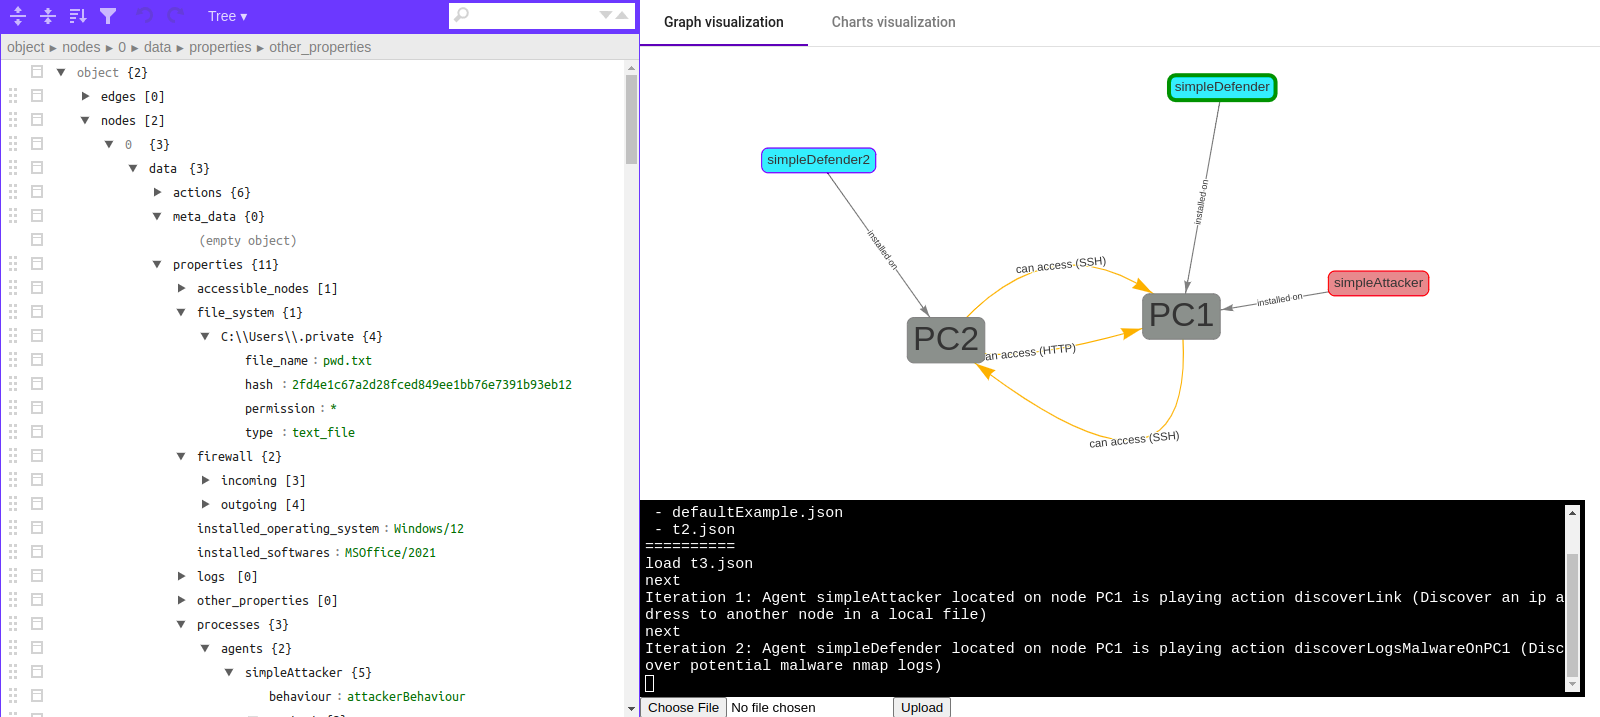
\includegraphics[width=0.9\linewidth]{images/interface_MCAS.png}
        \caption{Overview of MCAS}
        \label{fig:interface_simulateur}
    \end{figure}

    \vspace{-2ex}

    \item \headingNoLine{Collective strategies approaches}:
    \begin{itemize}
        \item \textbf{Multi-Agent Reinforcement Learning (MARL)}
        \item \textbf{(Distributed Constrained Optimization Problem)}
    \end{itemize}

\end{itemize}


\begin{figure}
    \centering
    % 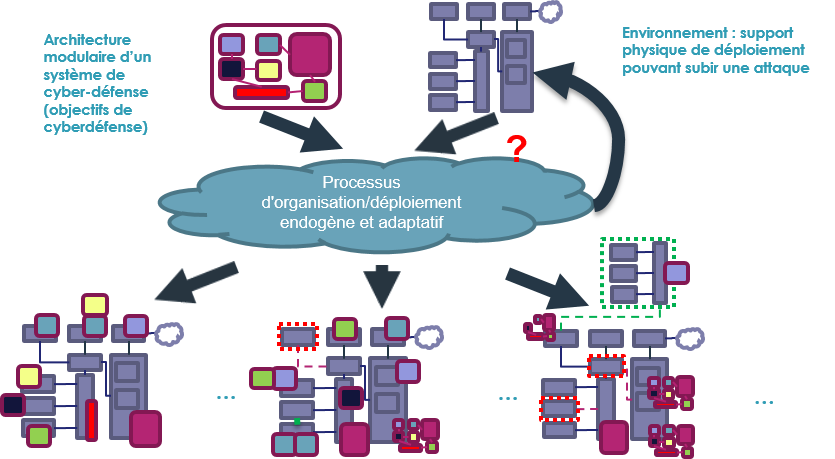
\includegraphics[width=0.9\columnwidth]{images/objectifs.png}
    \includesvg[width=0.73\columnwidth]{images/MARL_cyberdefense.svg}
    \caption{An MARL model view}
    \label{fig:my_label}
\end{figure}

% \vspace{-0.8ex}

% \begin{figure}
%     \centering
%     % 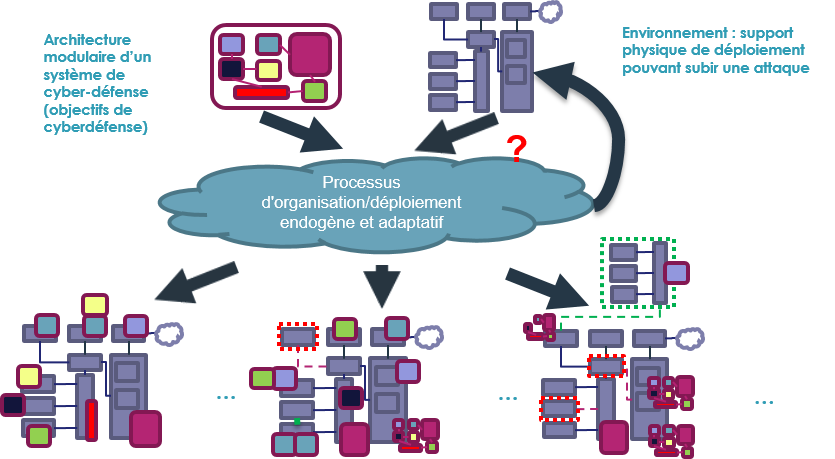
\includegraphics[width=0.9\columnwidth]{images/objectifs.png}
%     \includesvg[width=0.97\columnwidth]{images/DCOP.svg}
%     \caption{An DCOP model view}
%     \label{fig:my_label}
% \end{figure}

\vspace{-2ex}

% \begin{itemize}
%     \item \headingNoLine{Organization space exploration approach}
% \end{itemize}

\end{variableblock}

\begin{variableblock}{Conclusion: towards exploration of organization space}{bg=lightgray,fg=black}{bg=lightgray,fg=black}

\begin{figure}
    \raggedleft
    % 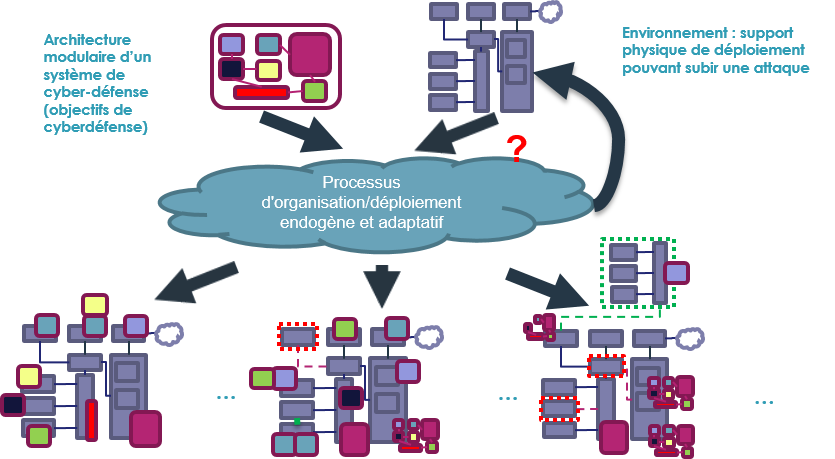
\includegraphics[width=0.9\columnwidth]{images/objectifs.png}
    \includesvg[width=0.7\columnwidth]{images/approche_organisation.svg}
\end{figure}

\end{variableblock}

% \begin{alertblock}{Conclusion}
% \begin{itemize}

% \item Overview of possible organizations respecting cyber-defense objectives and environmental constraints

% \item But not sufficient and need an experimental framework for the organization of a cyber-defense MAS in a network environment.
% \begin{itemize}
% \item To explore, evaluate and draw recommendations about the organization
% \end{itemize}

% \end{itemize}

% \end{alertblock}

% \begin{block}{References}
    
% % \nocite{*}
% % \footnotesize{\bibliographystyle{plain}\bibliography{local_references}}

% \vspace{-5ex}

% \begin{multicols}{2}[\frametitle{\insertsection} \usebeamertemplate{frametitle}]
% \bibliography{local_references}
% \bibliographystyle{plain}
% \end{multicols}

% \end{block}


\end{column}
\separatorcolumn



\end{columns}
\end{frame}

\end{document}

